\documentclass{beamer}

%%%%%%%%%%%%%Solarized Theme%%%%%%%%%%%%%%%
\usecolortheme[dark,accent=cyan]{solarized}
\beamertemplatenavigationsymbolsempty

%%%%%Packages%%%%%
\usepackage{graphicx}
\usepackage{hyperref}
\usepackage{colortbl, xcolor}
\usepackage{booktabs}
\usepackage{standalone}

\usepackage{tikz}
\usetikzlibrary{calc}

% Tick Boxes for itemize
\usepackage{enumitem}
\newlist{todolist}{itemize}{2}
\setlist[todolist]{label=$\square$}
\usepackage{pifont}
\newcommand{\cmark}{\ding{51}}%
\newcommand{\xmark}{\ding{55}}%
\newcommand{\done}{\rlap{$\square$}{\raisebox{2pt}{\large\hspace{1pt}\cmark}}%
\hspace{-2.5pt}}

%%%%%%Title%%%%%%%%
\title{\textbf{Machine learning and the Iterated Prisoner's Dilemma}}
\date{\\ \small{Dr. Vincent \textsc{Knight} \hspace{.5cm}  Dr. Jonathan \textsc{Gillard} }}
\institute[]
{\textbf{SECOND YEAR REPORT}}

\begin{document}

\maketitle 

\begin{frame}
    \begin{center}
    
\includegraphics[width=0.20\textwidth]{static/progress.pdf} \hspace{30pt}
    
\includegraphics[width=0.20\textwidth]{static/learn.pdf}
    \end{center}
\end{frame}

\begin{frame}
    \begin{center}
    
\includegraphics[width=0.20\textwidth]{static/progress.pdf} \hspace{30pt}
    \end{center}
\end{frame}

\begin{frame}
    \begin{center}
    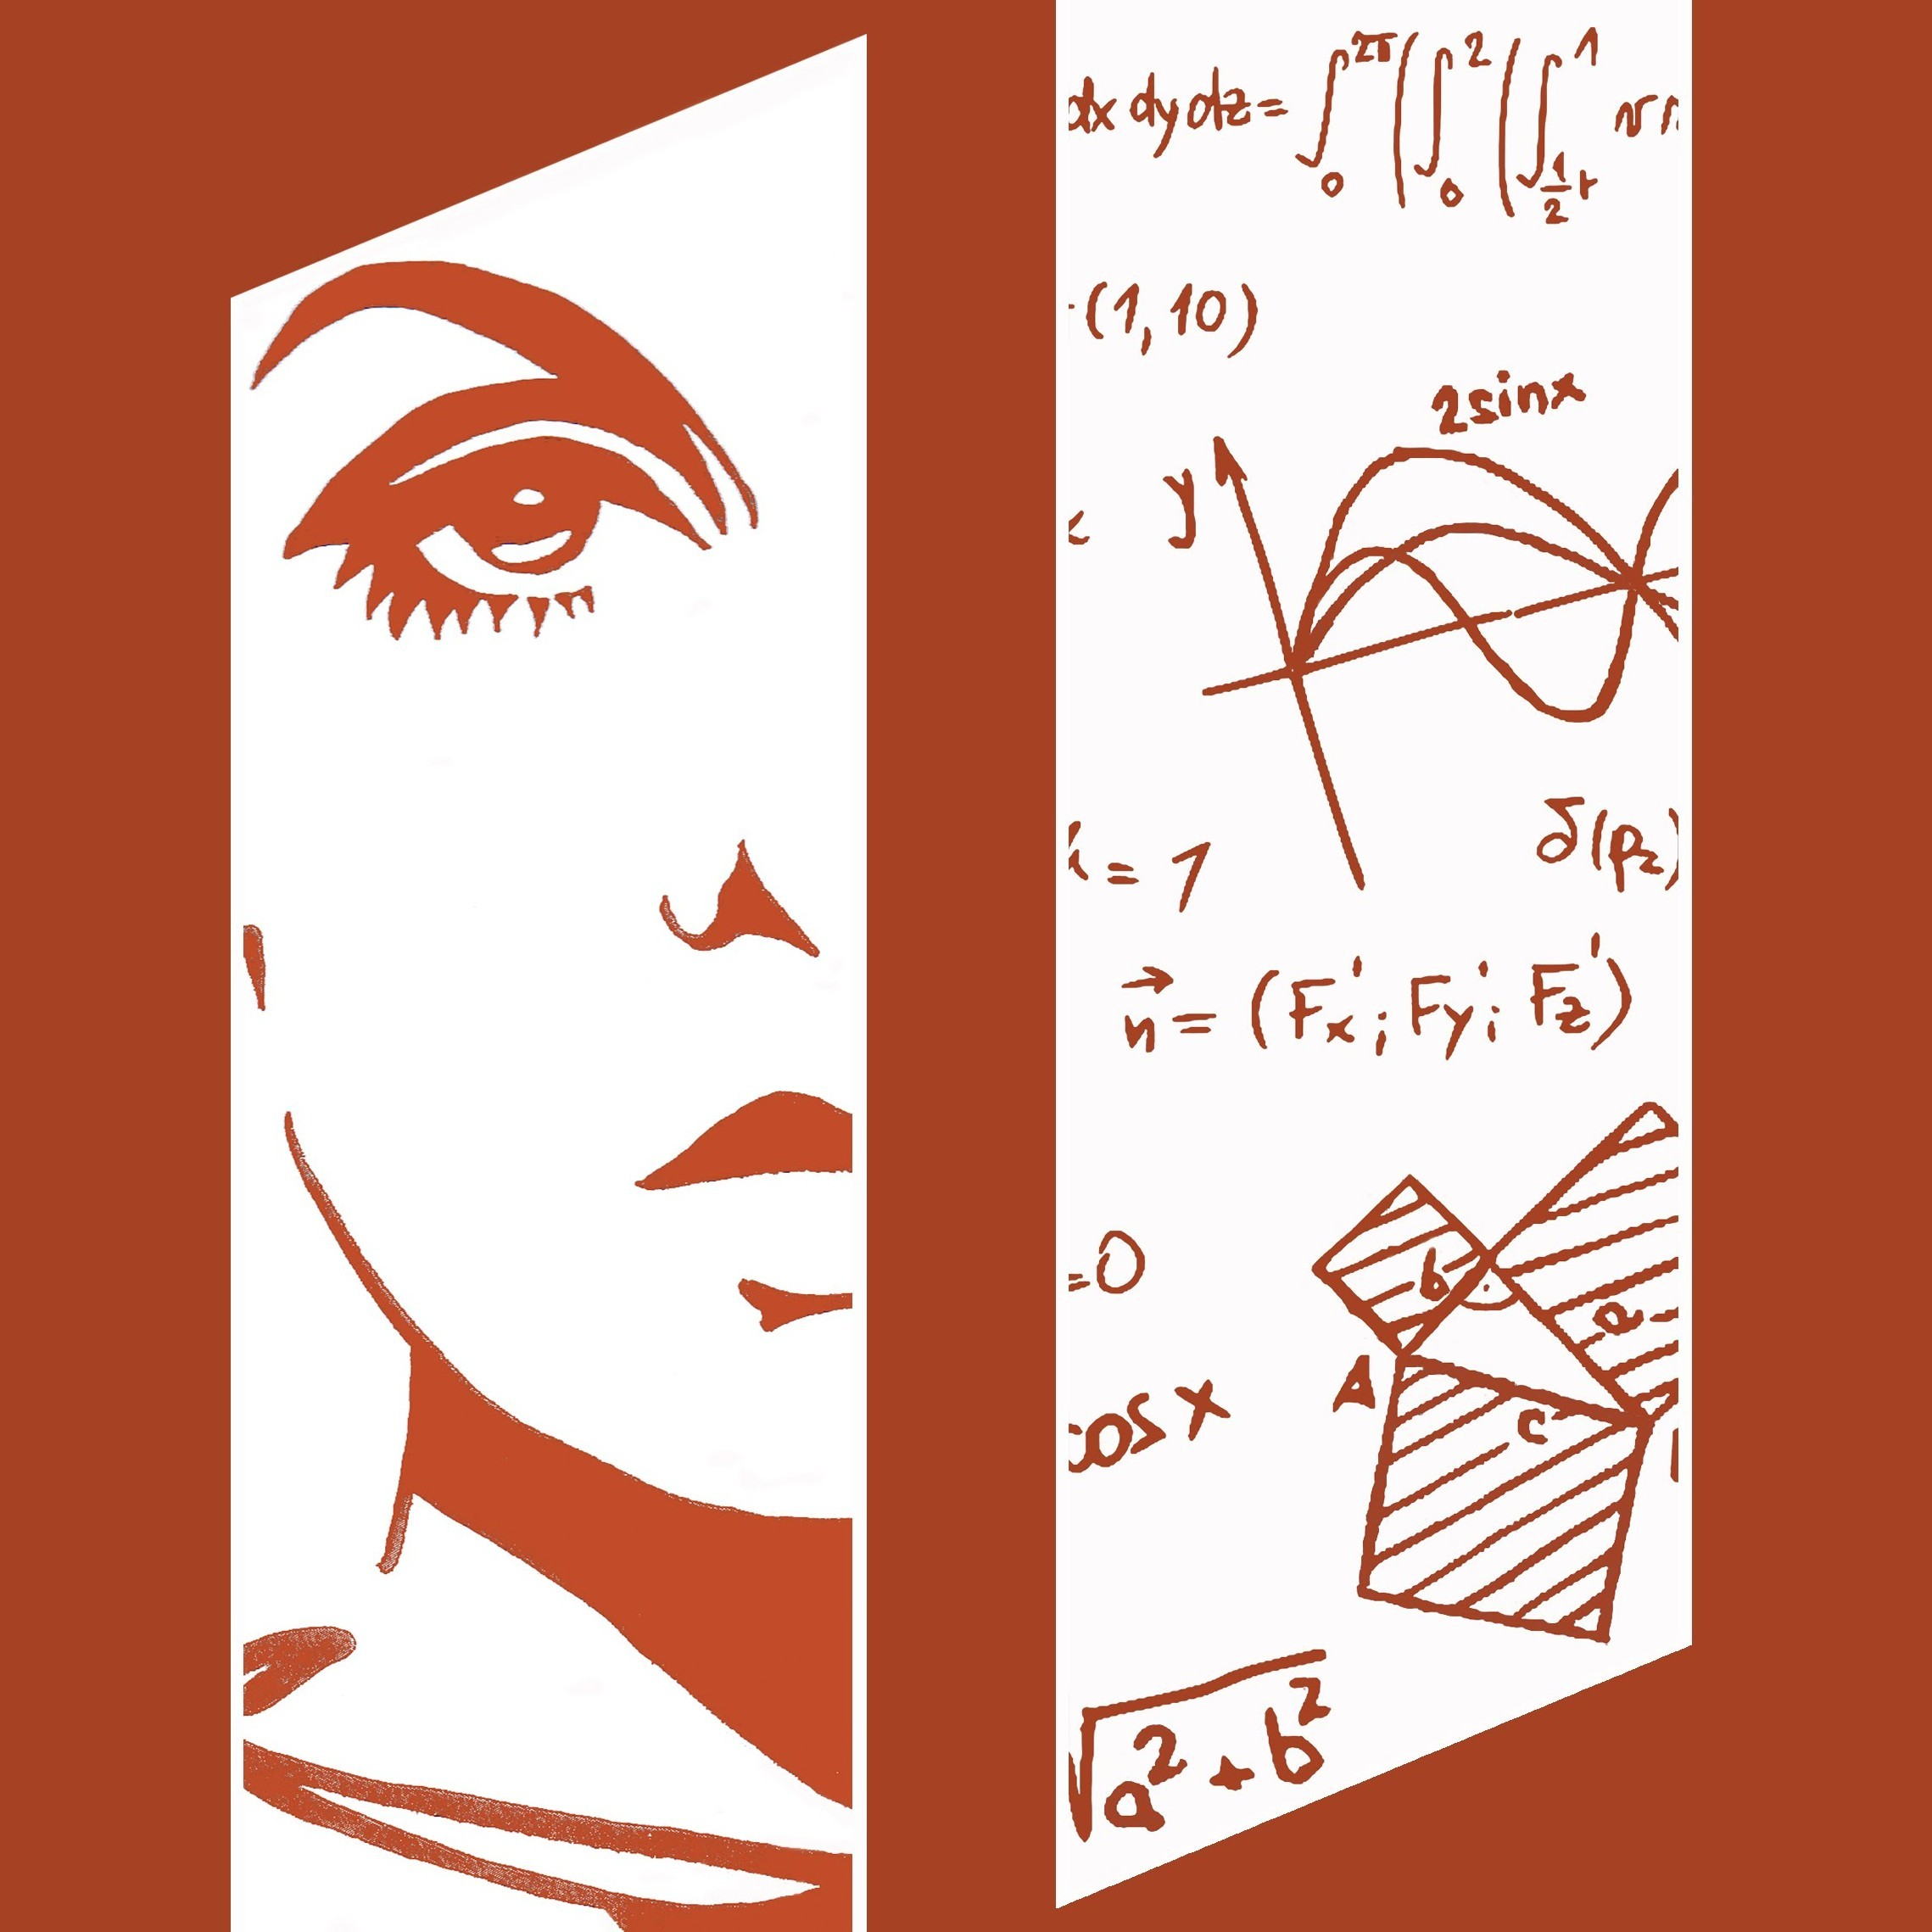
\includegraphics[width=0.3\textwidth]{static/wim.jpg}\hspace{10pt}
    
\includegraphics[width=0.3\textwidth]{static/plos.jpg}
    \vspace{10pt}

    
\includegraphics[width=0.3\textwidth]{static/soapbox.jpg} \hspace{10pt}
    
\includegraphics[width=0.3\textwidth]{static/emt.png}\vspace{10pt}
    \end{center}
\end{frame}

\begin{frame}
\small{
    \begin{center}
    \textcolor{orange}{
    \begin{todolist}
    \item[\done] \textbf{Reinforcement Learning Produces Dominant Strategies for the Iterated
    Prisoner's Dilemma}. PLOS One. 2017.
    \item \textbf{An Evolutionary Game Theoretic Model of Rhino Horn Devaluation}.
    Arxiv pre print. 2017. (under review with Ecological Modelling)
    \item \textbf{Evolution Reinforces Cooperation with the Emergence of Self-Recognition Mechanisms: an empirical study of the Moran process for the iterated Prisoner's dilemma}. Vincent Knight,
    Arxiv pre print. 2017. (under review with PLOS One)
    \end{todolist}}
    \end{center}}
\end{frame}

\begin{frame}
    \begin{center}
    
\includegraphics[width=0.20\textwidth]{static/learn.pdf}
    \end{center}
\end{frame}

\begin{frame}
    \begin{center}
    \textcolor{orange}{
    \begin{todolist}
        \item[\done] Machine Learning. Duration: \textbf{88 hours}.
        \item[\done] MA3600 Game Theory. Duration: \textbf{40 hours}.
        \item[\done] NATCOR Stochastic Modelling. Duration: \textbf{40 hours}.
        \item[\done] NATCOR Simulation. Duration: \textbf{40 hours}.
        \item[\done] NATCOR Combinatorial Optimisation. Duration: \textbf{40 hours}.
      \end{todolist}}
    \end{center}
\end{frame}

\begin{frame}
\centering
\Huge \textcolor{orange}{\textbf{Resultant Theory}}
\end{frame}

\begin{frame}
    \centering
    \includestandalone[width=0.8\textwidth]{static/resultant}
    \end{frame}

\begin{frame}
    {\Large
    \textcolor{orange}{
    \boldmath
    \begin{align*}
    f & = x ^ 2 - 5  x + 6 \\
    g & = x ^ 2 - 3  x + 2
    \end{align*}}
    \pause
    \textcolor{orange}{
    \boldmath
    \begin{align*}
    S = \left[\begin{matrix}1 & -5 & 6 & 0\\0 & 1 & -5 & 6\\1 & -3 & 2 & 0\\0 & 1 & -3 & 2\end{matrix}\right]\text{, where }
    det(S) = 0
    \end{align*}}}

\end{frame}

\begin{frame}
    {\Large
    \textcolor{orange}{
    \boldmath
    \begin{align*}
    f & = x ^ 2 + x  y + 2 x + y -1 \\
    g & = x ^ 2 + 3  x - y ^ 2 + 2  y - 1
    \end{align*}}
    \pause
    \textcolor{orange}{
     \boldmath\[S = \left[\begin{matrix}x + 1 & x^{2} + 2 x - 1 & 0\\0 & x + 1 & x^{2} + 2 x - 1\\-1 & 2 & x^{2} + 3 x - 1\end{matrix}\right]\]
    \pause
    \vspace{1cm}
     \boldmath\[det(S) = - x \left(x - 1\right) \left(x + 3\right)\]}}
\end{frame}

\begin{frame}
    \begin{center}
    \textcolor{orange}{\textbf{\Huge{
        Sylvester \\ \vspace{1cm}
        Bezout}}}
    \end{center}
\end{frame}

\begin{frame}
    \centering
    \textcolor{orange}{\textbf{\Huge{
        Macaulay \\ \vspace{1cm}
        Dixon }}}
\end{frame}

\begin{frame}
    \begin{center}
    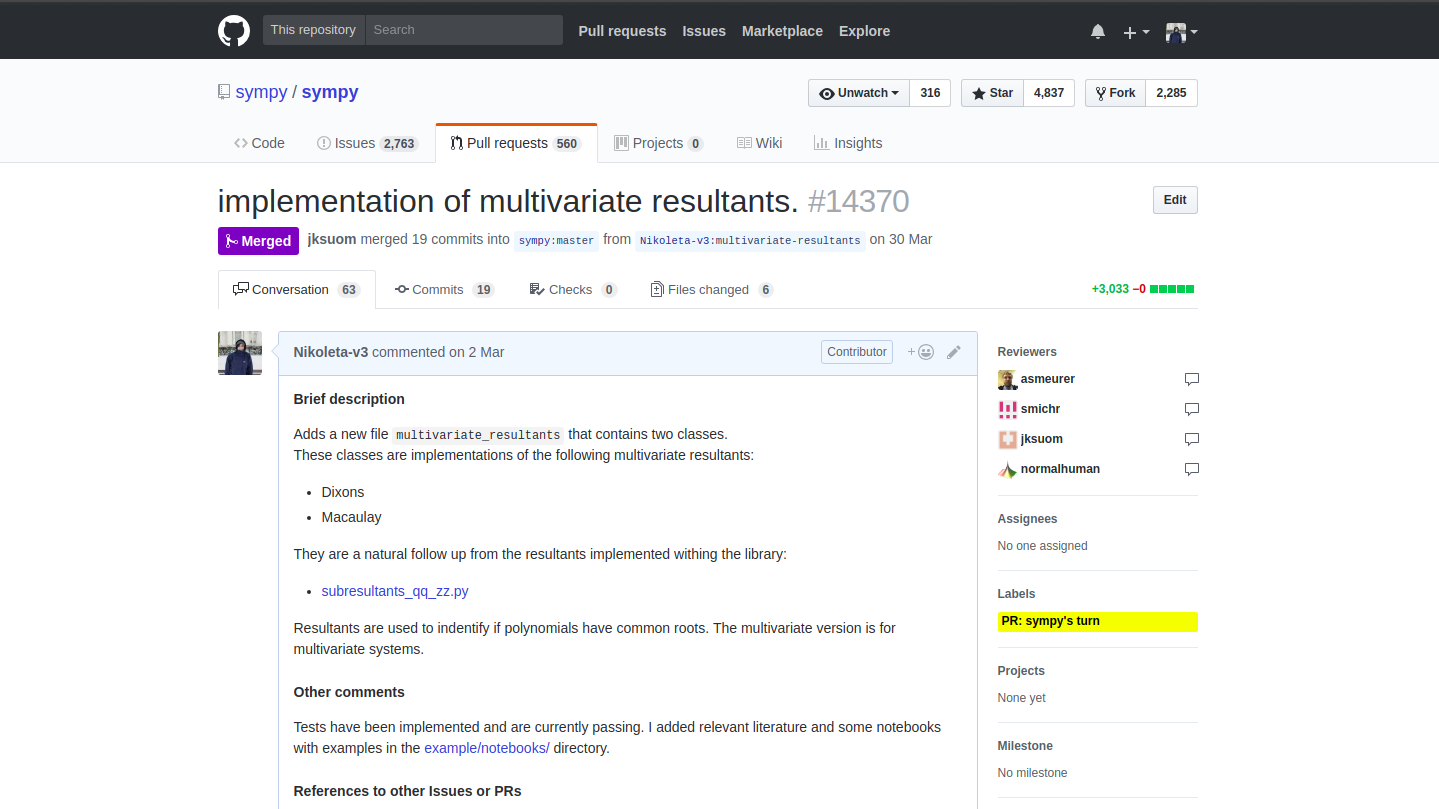
\includegraphics[width=\textwidth]{static/contribution.png}
    \end{center}
\end{frame}

\begin{frame}
	\begin{center}
		\Huge \textcolor{orange}{\textbf{Thank you!}}
	\end{center}
\end{frame}

\end{document}

